%
% This is a borrowed LaTeX template file for lecture notes for CS267,
% Applications of Parallel Computing, UCBerkeley EECS Department.
% Now being used for CMU's 10725 Fall 2012 Optimization course
% taught by Geoff Gordon and Ryan Tibshirani.  When preparing 
% LaTeX notes for this class, please use this template.
%
% To familiarize yourself with this template, the body contains
% some examples of its use.  Look them over.  Then you can
% run LaTeX on this file.  After you have LaTeXed this file then
% you can look over the result either by printing it out with
% dvips or using xdvi. "pdflatex template.tex" should also work.
%
\documentclass[twoside]{article}
\usepackage{graphicx}
\usepackage{tikz}
\usepackage{mathpazo}
\usetikzlibrary{decorations.pathmorphing}


\setlength{\oddsidemargin}{0.25 in}
\setlength{\evensidemargin}{-0.25 in}
\setlength{\topmargin}{-0.6 in}
\setlength{\textwidth}{6.5 in}
\setlength{\textheight}{8.5 in}
\setlength{\headsep}{0.75 in}
\setlength{\parindent}{0 in}
\setlength{\parskip}{0.1 in}
%
% ADD PACKAGES here:
%
\usepackage{amsmath,amsfonts,graphicx}
%
% The following commands set up the lecnum (lecture number)
% counter and make various numbering schemes work relative
% to the lecture number.
%
\newcounter{lecnum}
\renewcommand{\thepage}{\thelecnum-\arabic{page}}
\renewcommand{\thesection}{\thelecnum.\arabic{section}}
\renewcommand{\theequation}{\thelecnum.\arabic{equation}}
\renewcommand{\thefigure}{\thelecnum.\arabic{figure}}
\renewcommand{\thetable}{\thelecnum.\arabic{table}}
%
% The following macro is used to generate the header.
%
\newcommand{\lecture}[5]{
   \pagestyle{myheadings}
   \thispagestyle{plain}
   \newpage
   \setcounter{lecnum}{#1}
   \setcounter{page}{1}
   \noindent
   \begin{center}
   \framebox{
      \vbox{\vspace{2mm}
    \hbox to 6.28in { {\bf Physics 467/667: Thermodynamics/Statistical Physics
	\hfill Spring 2017} }
       \vspace{4mm}
       \hbox to 6.28in { {\Large \hfill Lecture #1: #2  \hfill} }
       \vspace{2mm}
       \hbox to 6.28in { {\it Lecturer: #3 \hfill Scribes: #4} }
      \vspace{2mm}}
   }
   \end{center}
   \markboth{Lecture #1: #2}{Lecture #1: #2}
   \vspace*{4mm}
}
%
% Convention for citations is authors' initials followed by the year.
% For example, to cite a paper by Leighton and Maggs you would type
% \cite{LM89}, and to cite a paper by Strassen you would type \cite{S69}.
% (To avoid bibliography problems, for now we redefine the \cite command.)
% Also commands that create a suitable format for the reference list.
\renewcommand{\cite}[1]{[#1]}
\def\beginrefs{\begin{list}%
        {[\arabic{equation}]}{\usecounter{equation}
         \setlength{\leftmargin}{2.0truecm}\setlength{\labelsep}{0.4truecm}%
         \setlength{\labelwidth}{1.6truecm}}}
\def\endrefs{\end{list}}
\def\bibentry#1{\item[\hbox{[#1]}]}
%Use this command for a figure; it puts a figure in wherever you want it.
%usage: \fig{NUMBER}{SPACE-IN-INCHES}{CAPTION}
\newcommand{\fig}[3]{
			\vspace{#2}
			\begin{center}
			Figure \thelecnum.#1:~#3
			\end{center}
	}
% Use these for theorems, lemmas, proofs, etc.
\newtheorem{theorem}{Theorem}[lecnum]
\newtheorem{lemma}[theorem]{Lemma}
\newtheorem{proposition}[theorem]{Proposition}
\newtheorem{claim}[theorem]{Claim}
\newtheorem{corollary}[theorem]{Corollary}
\newtheorem{definition}[theorem]{Definition}
\newenvironment{proof}{{\bf Proof:}}{\hfill\rule{2mm}{2mm}}
% **** IF YOU WANT TO DEFINE ADDITIONAL MACROS FOR YOURSELF, PUT THEM HERE:
\newcommand\E{\mathbb{E}}
\begin{document}
%FILL IN THE RIGHT INFO.
%\lecture{**LECTURE-NUMBER**}{**DATE**}{**LECTURER**}{**SCRIBE**}
\lecture{11}{Entropy and Heat}{Qiang Zhu}{scribe-name1,2,3}
%\footnotetext{These notes are partially based on those of Nigel Mansell.}
% **** YOUR NOTES GO HERE:
% Some general latex examples and examples making use of the
% macros follow.  
%**** IN GENERAL, BE BRIEF. LONG SCRIBE NOTES, NO MATTER HOW WELL WRITTEN,
%**** ARE NEVER READ BY ANYBODY.

\section{Some useful equations} % Don't be this informal in your notes!
\begin{equation} \label{idealgas} PV = nRT = NkT \end{equation}
\begin{equation} \label{Avogadro} N = n \times N_A \end{equation}
\begin{equation} \label{PV-micro} PV = Nm{\overline v_x^2} = NkT\end{equation}
\begin{equation} \label{eqpartition} U_{thermal} = N \cdot f \cdot \frac{1}{2}kT \end{equation}
\begin{equation} \label{1stlaw} \Delta{U} = Q + W \end{equation}
\begin{equation} \label{work3} \Delta W = - P \Delta{V} \end{equation}
\begin{equation} \label{entropy} S = k \text{ln}\Omega \end{equation}
\begin{equation} \label{entropy} dU = TdS - PdV \end{equation}

\section{Chemical Potential}
When we talk a system of Ideal gas), it is decribed by the following fundamental parameters, $T,P,N$,
\begin{enumerate}
\item uneven $T$ $\rightarrow$ heat     flow ($S \uparrow$), we call it {\it thermal equilibrium}
\item uneven $P$ $\rightarrow$ pressure flow ($S \uparrow$), we call it {\it mechanical equilibrium}
\item uneven $N$ $\rightarrow$ particle flow ($S \uparrow$), we call it ~~~~~~~~~~~~~?
\end{enumerate}
\begin{figure}[h]
\centering
\begin{tikzpicture}[thick]
\draw (0,0.4) -- (8,0.4) -- (8,4) -- (0,4) -- (0,0.4);
\draw (0.2,0.6) -- (4.4,0.6) -- (4.4,3.8) -- (0.2,3.8) -- (0.2,0.6);
\node at (1.8,2.8) {$U_A, N_A, S_A$};
\node at (1.8,2.2) {$P_A$};
\draw (7.8,0.6) -- (4.6,0.6) -- (4.6,3.8) -- (7.8,3.8) -- (7.8,0.6);
\node at (6.2,2.8) {$U_B, N_B, S_B$};
\node at (6.2,2.2) {$P_B$};
\draw [->,decorate,decoration=snake] (3.8,2) -- (5.0,2) node [above, xshift=-0.8cm]{particle flow};
\end{tikzpicture}
\caption{A schematic particle flow between two gases.}
\end{figure}

Such process due to the exchange of particles is called {\it diffusion}. Since diffusion is also a
spontaneous process. It must lead to the increase of entropy (recall we have learned the mixing entropy).
This indicates that $S$ is also a function of $N$ (as we learned in Chapter 2).
Therefore, we can also derive the equilibrium condition for diffusion (analogy to $P$).
\begin{equation} \label{entropy} 
\frac {\partial{S_A}} {\partial{N_A}} =  \frac {\partial{S_B}} {\partial{N_B}} 
\end{equation}

What's the physical meaning of $\partial{S_A}/\partial{N_A}$? \\
If we dig a bit on the units, we will find $\partial{S_A}/\partial{V_A}$ has a unit of J/K. 
Not a very pleasant quantity. Let's multiply it by $-T$ so that it has the dimension of energy.
\begin{equation} \label{entropy} 
\mu = -T (\frac {\partial{S}} {\partial{N}})_{U,V}
\end{equation}

So it means the equilibrium condition for diffusive process is $\mu_A$ = $\mu_B$.

Now let's we generalize the processes which I shown in the beginning.
\begin{enumerate}
\item uneven $T(\frac {\partial{S}} {\partial{U}} = 1/T)  $ $\rightarrow$ heat     flow ($S\uparrow$) , we call it {\it thermal equilibrium.}
\item uneven $P(\frac {\partial{S}} {\partial{V}} = P/T)  $ $\rightarrow$ pressure flow ($S\uparrow$) , we call it {\it mechanical equilibrium.}
\item uneven $N(\frac {\partial{S}} {\partial{N}} = \mu/T)$ $\rightarrow$ particle flow ($S\uparrow$) , we call it {\it diffusive equlibrium.}
\end{enumerate}

\section{The Generalized Thermodynamic Identity}

\begin{equation} dS = (\frac{\partial S}{\partial U})dU 
                    + (\frac{\partial S}{\partial V})dV  
                    + (\frac{\partial S}{\partial N})dN 
\end{equation}
\begin{equation} dS = \frac{1}{T}dU
                    + \frac{P}{T}dV  
                    - \frac{\mu}{T}dN
\end{equation}
\begin{equation} dU = TdS - PdV  + \mu dN\end{equation}
\begin{enumerate}
\item $\Delta{U,V}=0$, $\mu$=
\item $\Delta{S,V}=0$, $\mu$=
\end{enumerate}
$\mu$ is the system's energy change when you add one particle while $S$ and $V$ is fixed. Normally, $\mu$ is negative.\\
\begin{figure}[h]
\centering
\begin{tikzpicture}
\draw (2,0) circle (0.4cm);
\draw (2.5,-0.5) -- (2.5,0.5);
\draw (3,0) circle (0.4cm);
\draw (4,0) circle (0.4cm);
\draw (4.5,-0.5) -- (4.5,0.5);
\draw (5.5,-0.5) -- (5.5,0.5);
\draw (3.5,-1.0) node [below] {$N$=3, $q$=3, $\Omega$=10};
\draw [->] (7.0,0.0) -- (10.0,0.0);
\draw (12,0) circle (0.4cm);
\draw (12.5,-0.5) -- (12.5,0.5);
\draw (13,0) circle (0.4cm);
\draw (13.5,-0.5) -- (13.5,0.5);
\draw (14.5,-0.5) -- (14.5,0.5);
\draw (15.5,-0.5) -- (15.5,0.5);
\draw (13.5,-1.0) node [below] {$N$=4, $q$=2, $\Omega$=10};
\end{tikzpicture}
\end{figure}


For Einstein solid, $\mu$=-$\epsilon$\\
For a more realistic example, let's do ideal gas of He (0.32 eV, how to calculate?)
\begin{enumerate}
\item Can we make an isotropic process.
\item No diffusion Einstein Solid.
\item No diffusion between two He gases.
\item generalized equation
\begin{equation} dU = TdS - PdV  + \sum_{\substack{i}} \mu_i dN_i\end{equation}
\end{enumerate}


\section{Homework}
Problem 3.36, 3.37, 3.38


\end{document}

